\chapter{Functionality}\label{ch:functionality}

The GUI's complete functionality is organized across multiple specialized windows. To properly access all features, always launch the application through \texttt{main.mlapp} and access other windows from within this main interface. The following sections detail each component.

\section{Main Interface: \texttt{main.mlapp}}

This primary interface allows users to:
\begin{itemize}
    \item Configure various simulation parameters
    \item Adjust plot settings
    \item Import existing datasets
    \item Generate files for batch processing
\end{itemize}

At the top of the interface (shown in Figure \ref{fig:main1}), you'll find three key controls:

\begin{itemize}
    \item \textbf{Plot Button}: Initiates new simulations. Detail see in Section~\ref{sec:new_run}. **\textit{Important}: Do not use this button for visualizing existing datasets.
    
    \item \textbf{Mode Selection Dropdown}: Offers two operational modes:
    \begin{itemize}
        \item \textit{Run Mode}: Single execution with one $W_S$ value through the entire time course.
        \item \textit{Stimulation Mode}: Multiple executions with various $W_s$ values, potentially repeating the time course.
    \end{itemize}
    
    \item \textbf{Quit Button} (grayed out initially): Becomes active only after starting a simulation and remains available until completion.
\end{itemize}

\begin{figure}[H]
    \centering
    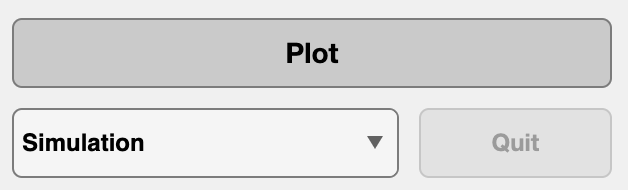
\includegraphics[width=0.35\textwidth]{figs/mainapp1.png}
    \caption{Main interface controls showing the Plot button, mode selector, and Quit button.}
    \label{fig:main1}
\end{figure}

\subsection{General Settings}
Under the Setting tab, you can adjust values using the sliders or by directly entering desired values into the editable fields with a white background. Fields with a gray background are read-only and are automatically calculated based on other variables.

\begin{itemize}
    \item \textbf{Choice Number:} Specifies the number of available decision alternatives in the simulation.
    
    \item \textbf{Total Time:} Defines the duration of each simulation run.
    
    \item \textbf{Block Number:} Determines the number of distinct reward conditions per simulation. During reward switching, probabilities/magnitudes undergo circular shifting with random shift values, ensuring the new condition never matches the previous one.
    
    \item \textbf{Tau ($\tau$):} Time constant governing the decay rate of the reward rate estimator.
    
    \item \textbf{Self-excitation Weight ($W_s$):} Controls the self-excitation strength for reward rate estimators across the $n$ choices.
    
    \item \textbf{Effective Time Constant ($\tau'$):} Derived parameter calculated as $\tau' = \tau/(1-W_s)$, representing the modified time constant accounting for self-excitation.
    
    \item \textbf{Time Step (dt):} Discrete time increment used for numerical simulation.
    
    \item \textbf{Sessions:} For batch processing, specifies the number of independent simulations performed with identical parameter settings.
    
    \item \textbf{Initial Action Rate:} Sets the starting value for the action rate at simulation onset.
    
    \item \textbf{Initial Reward Rate:} Defines the initial reward rate estimate at the beginning of the simulation.
    
    \item \textbf{Arbitrary Decision:}​​ This feature allows you to enforce a specific decision at any given time, overriding the system's normal decision-making process. The desired choice is specified in the provided text area, following the format described in Section~\ref{sec:text_area}. To apply the same choice to all designated time points, simply enter a single choice value.
\end{itemize}

\subsection{Random Walk}
Defines the movement of a simulated dot (\(\mathbf{V}_t\)) with the following stochastic differential equation:  
% \[dV_t = \mu(V_\alpha(n), R_t) dt + \sigma dW_t\]
\[d\mathbf{V}_t =  (\lambda \mathbf{V}_t + \rho \mathbf{R}_t) \ dt + \sigma \ d\mathbf{W}_t\]
where \(\mu(V_\alpha(n), R_t, c_\mu)\) is the drift function given by:
% \[
% \mu(V_\alpha(n), R_t, c_\mu) = c_\mu V_\alpha(n) \times R_t
% \]
% {\color{red} \textit{Maybe like this? Also, since we are talking about vectors, vectors should be bolded; scalars can be left in regular math font; and the $\times$ symbol means "cross product" in vector notation so replace by $\cdot$. Also, I don't think we even need a separate $\mu$ function -- see my alternative equation above. Are you including $V_t$ as the equivalent of Threshold-v in the code? }}

\[\mu(\mathbf{V}_t, \mathbf{R}_t) = c_\mu  \mathbf{R}_t\]

Here:
\begin{itemize}
    \item \(\mathbf{V}_t\) represents the state variable (the position of the decision particle) as a column vector in $n$ dimensions for $n$ choices
    \item \(\mathbf{R}_t\) is the vector of the agent's reward rate estimates for each choice at time \(t\), also a column vector of $n$ rows
    \item $\rho$ is a scaling constant for the drift, called "Drift Constant" in the app
    \item \(\mathbf{W}_t\) is a Wiener process (standard Brownian motion).
\end{itemize}

This continuous-time system is simulated in discrete time, with time step size of $\Delta t$, as follows:
\[\mathbf{V}_{\mathrm{new}} = \mathbf{V}_\mathrm{old} + \Delta t \cdot (\lambda\mathbf{V}_t + \rho \mathbf{R}_t) + \sigma \,\sqrt{\Delta t} \, N(0,1) \]
where $N(0,1)$ refers to a standard normal random variable

If the dot crosses a threshold, the model treats it as a decision. Thresholds \(\alpha\) are calculated using:
\[
\alpha(d, \mathbf{R}_t, \alpha_m) = 
\min\left(\frac{d}{\max(\mathbf{R}_t, 0)}, \alpha_m\right)
\]
\[\theta_i(d,\mathbf{R}_{t_i},\theta_m) = \mathrm{min} \left( \frac{d}{\mathrm{max}(\mathbf{R}_{t_i},0)}, \theta_m \right)\]
where:
\begin{itemize}
    \item \(d\) is the threshold scaling parameter.
    \item \(\mathbf{R}_t\) is the reward at time \(t\), with \(\max(\mathbf{R}_t, 0)\) ensuring that the reward is non-negative.
    \item \(\alpha_m\) is the maximum allowable threshold.
\end{itemize}
A choice that is not selected for an extended period results in its reward rate approaching zero, causing its threshold distance to approach infinity. To mitigate this, a maximum threshold distance is set relative to the starting coordinate to prevent instability during reward switches.

\subsection{Boredom Function}
\texttt{Reward Type} drop down allows selection of the reward mode:
    \begin{itemize}
        \item \textbf{Value 1:} Probability Mode – The probability of receiving a reward (magnitude = 1) depends on the Boredom function.
        \item \textbf{Value 3:} Magnitude Mode – The decision always yields a reward, but its magnitude is determined by the Boredom function.
    \end{itemize}

The reward probability or magnitude \(\mathbf{B}\) is defined as:
\[	
\mathbf{B}(k, \mathbf{A}(x), b) = \min\left(-k \mathbf{A}_t + b, B_{\min} \right)
\]
where the Action Rate \(\mathbf{A}_t\) evolves over time according to the following dynamics:
\[
\mathbf{A}_{t+ \Delta t} = 
\begin{cases}
    \dfrac{1}{\tau} (1 - W_s) \left[ 1 - \mathbf{A}_t \Delta t \right], 
    & \text{if } V_t \geq \alpha, \\[12pt]
    -\dfrac{1}{\tau} (1 - W_s) \mathbf{A}_t \Delta t, 
    & \text{if } V_t < \alpha.
\end{cases}
\]
You can enter multiple values for \(k\), individual \(b\), or minimum probability or magnitude values in their respective text fields, separated by commas.

For the \texttt{Max \& Min} option in the \(b\) dropdown, the values of \(b\) will be distributed evenly between the minimum and maximum based on the number of choices.  
\begin{itemize}
    \item \textbf{\(b\) Type 1: Max \& Min.} When selecting this option, you can enter the maximum and minimum values for \(b\), and the system will automatically generate evenly distributed \(b\) values based on the specified number of choices.
    \item \textbf{\(b\) Type 3: Individual values.} In this case, you can manually input individual \(b\) values, separated by commas.
\end{itemize}

The corresponding Boredom Function will be plotted under \texttt{BFGraph} tab. You can use this plot to verify and adjust the settings.

\begin{figure}[H]
    \centering
    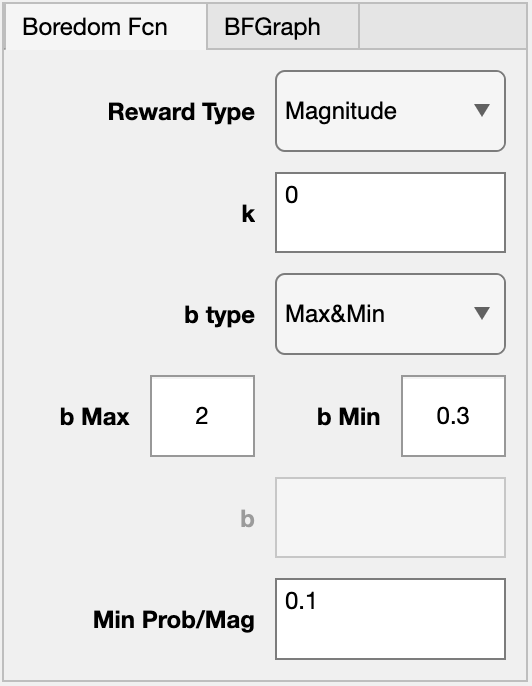
\includegraphics[width=0.5\textwidth]{figs/boredom_function_example.png}
    \caption{Sample Boredom Function Configuration. The plotted function will help verify the entered settings.}
    \label{fig:boredom_function_example}
\end{figure}

\subsection{Cost}
The cost function can be either linear or nonlinear, as defined by the following equations:

\[
\mathcal{C}(T, k_\mathcal{C}, c_\mathcal{C}) = 
\begin{cases}
    \dfrac{c_\mathcal{C}}{T}, & \text{(Linear case)} \\[15pt]
    \dfrac{k_\mathcal{C}}{T - c_\mathcal{C}}, & \text{(Nonlinear case).}
\end{cases}
\]

where \(T\) is the decision time, and \(k_\mathcal{C}\), \(c_\mathcal{C}\) are parameters that shape the cost function.

To switch between the two cost functions, click the corresponding checkbox. The cost function will be plotted under the \texttt{CGraph} tab for visual reference.

\begin{figure}[H]
    \centering
    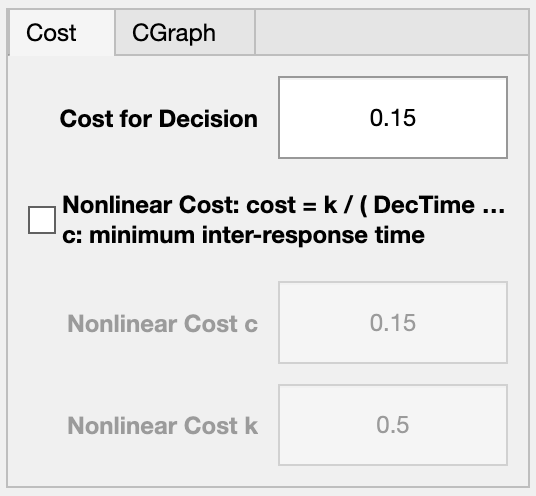
\includegraphics[width=0.5\textwidth]{figs/cost_settings.png}
    \caption{Sample Cost Function Settings.}
    \label{fig:cost_settings}
\end{figure}

\subsection{Timer}

The timer dynamics follow a random walk, which can be described in two cases:

\[
d\mathcal{T} = \sigma_\mathcal{T} d\bar{W}_t +
\begin{cases}
    \mu_\mathcal{T}^c dt , & \text{(non-adapting)} \\[15pt]
    \mu_\mathcal{T}(c_\mathcal{T},k_\mathcal{T}) dt , & \text{(adapting)}
\end{cases}
\]

where \( \mu_\mathcal{T}(c_\mathcal{T},k_\mathcal{T}) \) is the adaptation function, given by:

\[
\mu_\mathcal{T}(c_\mathcal{T},k_\mathcal{T}) = \max\left(\frac{1}{c_\mathcal{T}} - \frac{1}{k_\mathcal{T}\max\left(R_t, 0\right) + c_\mathcal{T}}, \mu_{\mathcal{T}_{\min}}\right)
\]

This function models the timer's dynamics, allowing it to adapt to the reward function \( R_t \). 

In the **\textbf{non-adapting}** case, the timer evolves at a constant rate determined by \( \mu_\mathcal{T}^c \). In the **\textbf{adapting}** case, the timer rate depends on the reward function \( R_t \) and two additional parameters, \( c_\mathcal{T} \) and \( k_\mathcal{T} \), which control the speed of adaptation. This ensures the timer dynamically adjusts to variations in the reward function, providing a more responsive system. The graph of the relationship between sum of reward rate and timer drift is depicted under the \texttt{ATGraph} tab.

A **\textbf{crossing}** in the timer's random walk results in a **\textbf{timeout}**, indicating that the decision process has reached its time limit.

The **\textbf{timeout boosting}** feature allows the system to shrink the thresholds by scaling them down by a common factor whenever a timeout occurs. This ensures that decisions are made within a reasonable time frame, particularly in the case of prolonged inaction.

\begin{figure}[H]
    \centering
    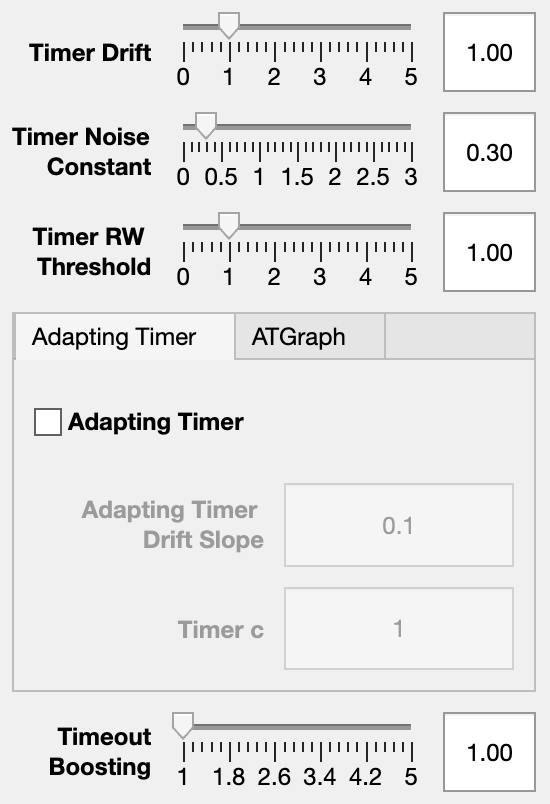
\includegraphics[width=0.5\textwidth]{figs/timer_settings.png}
    \caption{Sample Timer Settings.}
    \label{fig:timer_settings}
\end{figure}

\section{Running new Run/ Simulation and Plot} \label{sec:new_run}

To initiate a new simulation, click the \texttt{Plot} button located at the top of the main interface. This action will open a new window showing the plotted results.

On the top of the new window (shown in Figure \ref{fig:new_run_win}), you will find a status lamp that indicates the current state of the simulation (See Section~\ref{sec:status_lamp} for details). The \texttt{Quit} button will become active once the simulation starts and will remain available until the simulation is complete. Progress gauges will display the completion status of the current session and the overall batch process. Simulation time will be shown in the upper-right corner.

Below the status indicator, you will find two tabs: \texttt{Run} and \texttt{Simulation}. This GUI won't automatically adjust to the tab you are on when you click the \texttt{Plot} button. Please make sure you redirected to the correct tab to view the results you want.

\begin{figure}[H]
    \centering
    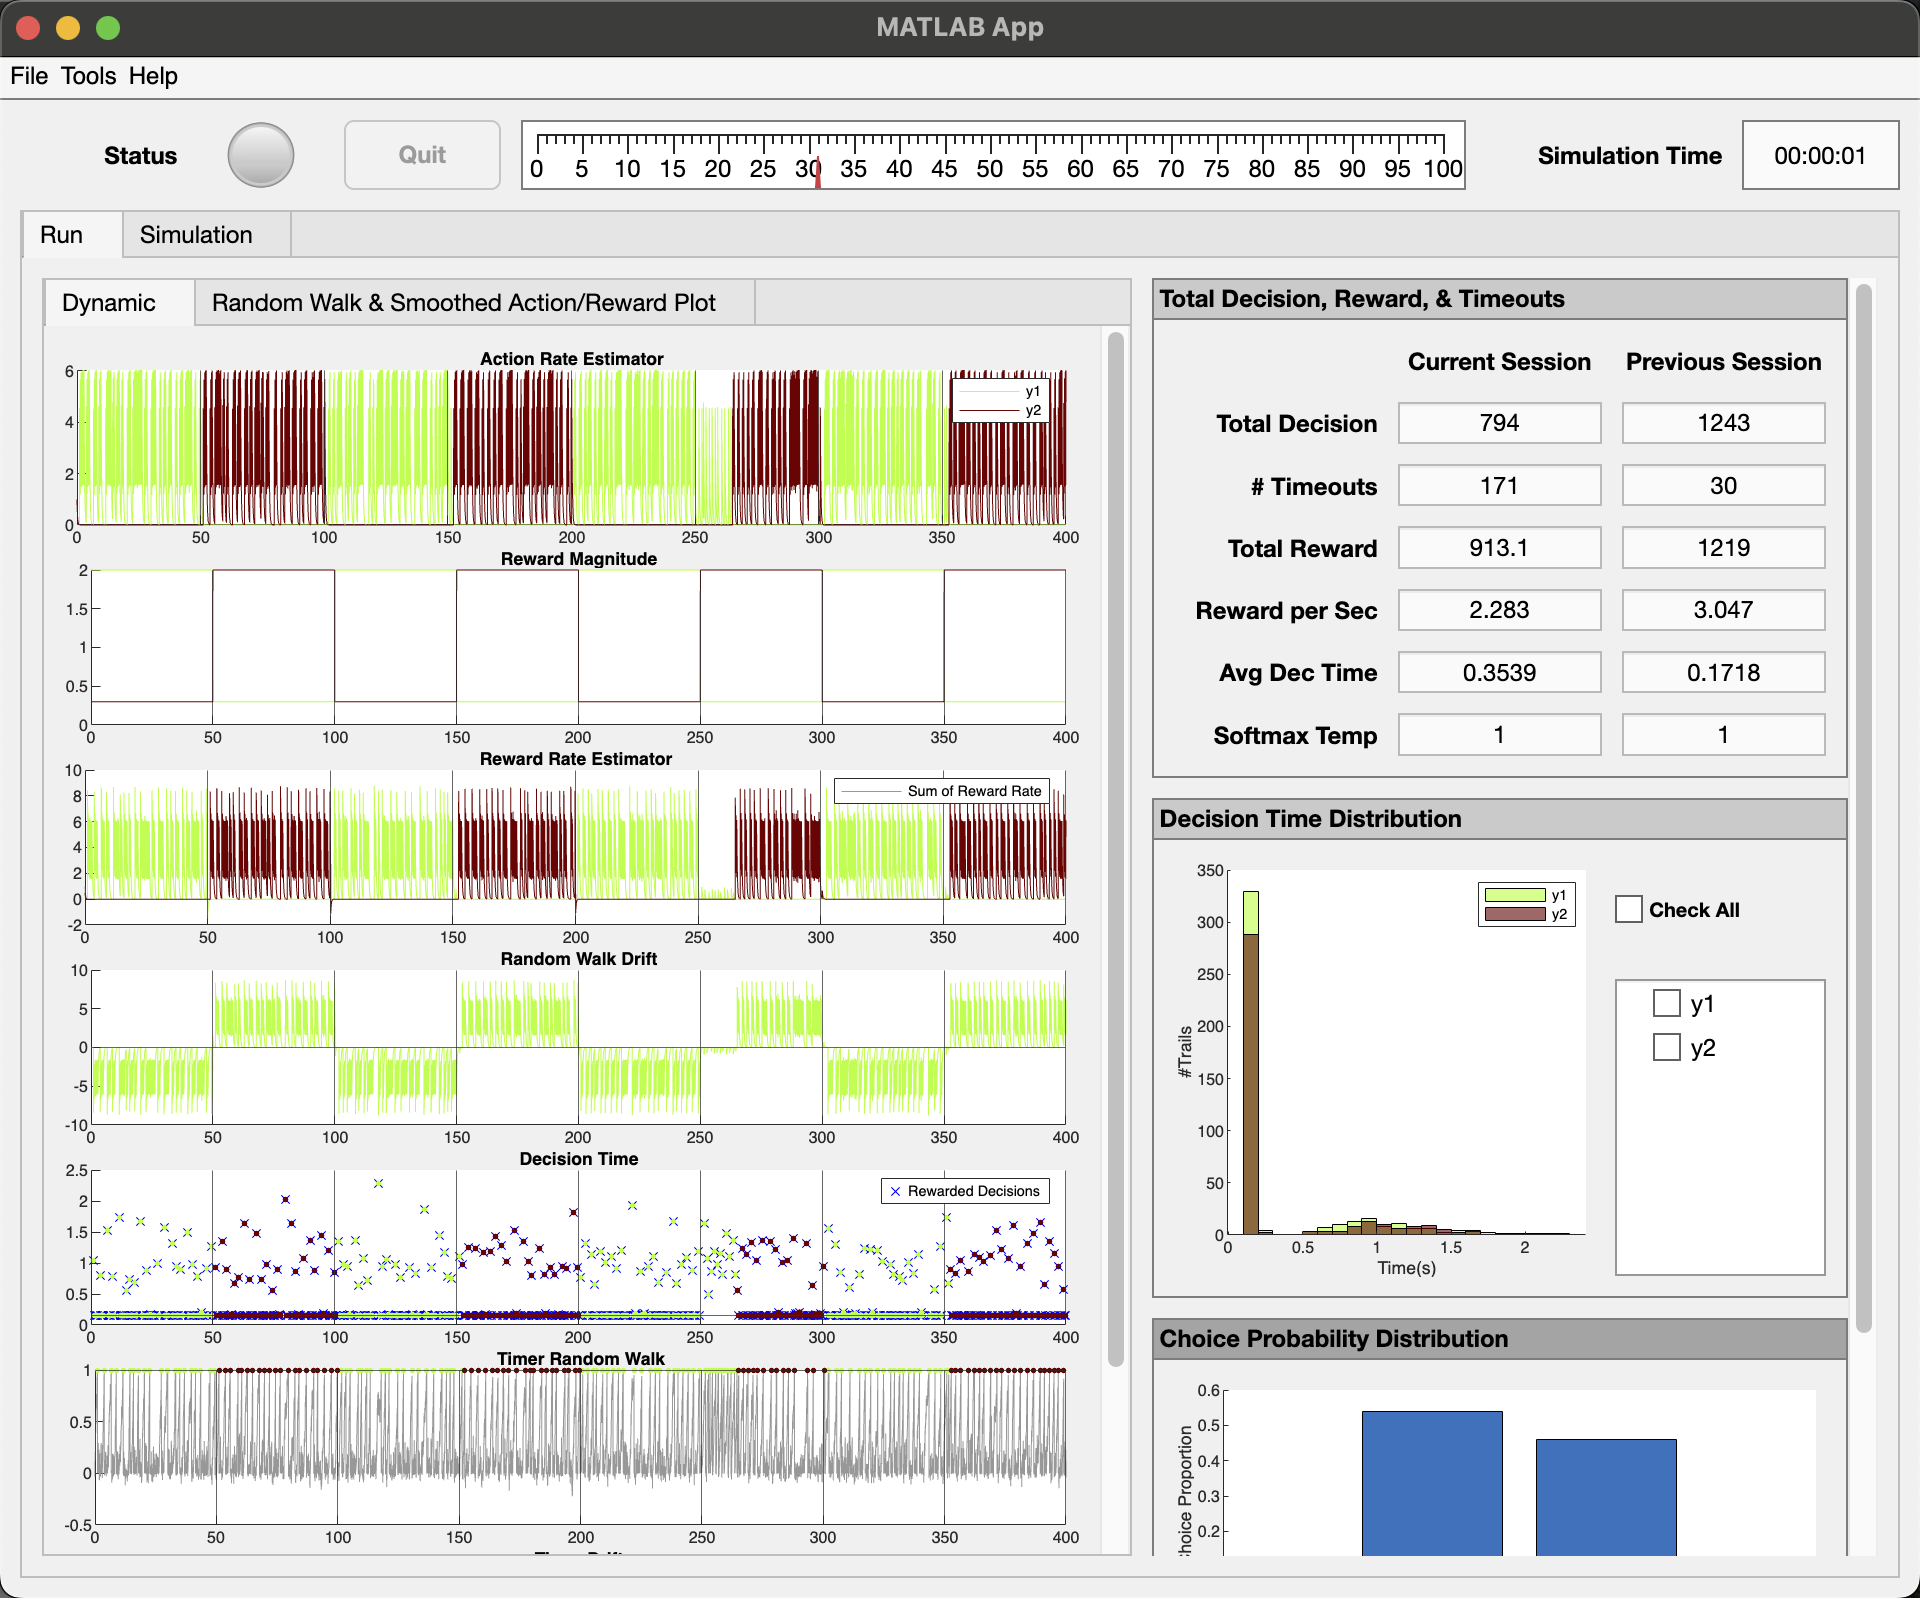
\includegraphics[width=\textwidth]{figs/new_run_win.png}
    \caption{Sample New Run Window.}
    \label{fig:new_run_win}
\end{figure}

\section{Importing Datasets for Visualization}

To import a simulated dataset or utilize existing datasets for plotting, navigate to the \texttt{File} $\rightarrow$ \texttt{Import Datasets} tab located in the upper-left corner of the GUI. This will direct you to open new windows for data import, where you can manage datasets for your visualization tasks.

\begin{figure}[H]
    \centering
    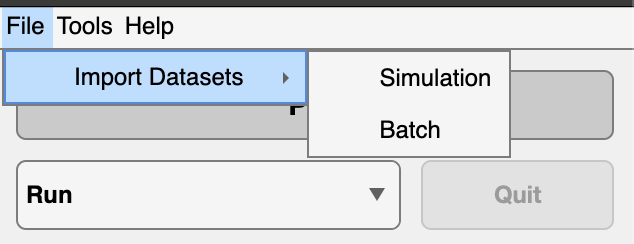
\includegraphics[width=0.5\textwidth]{figs/import_data.png}
    \caption{Click on this tab to go to saving \& importing page.}
    \label{fig:saving_n_import_tab}
\end{figure}

\subsection{Import Simulation} \label{sec:import_sim}

To import existing simulation from a dataset, nativate to the \texttt{File} $\rightarrow$ \texttt{Import Datasets} $\rightarrow$ \texttt{Simulation} tab. No setting adjusting can be done in this window. The upper \texttt{Settings} text area will show all the setting copy from your \texttt{main.mlapp} settings when you initially open this window. These will be the criteria for filtering datasets for import. Only the dataset comtaining the exactly same settings will be importted. Simply click on the \texttt{Import Files} button and select a directory to complete import. Note that this won't go through the file under subfolder.

When there's some files successfully imported, both \texttt{Clear All Files} and \texttt{Plot} button will be available. You may click on \texttt{Clear All Files} button to clear all the datasets you imported. Clicking on \texttt{Plot} button will lead to open another window for plotting using existing datasets. See Section *** for more detail.

\begin{figure}[H]
    \centering
    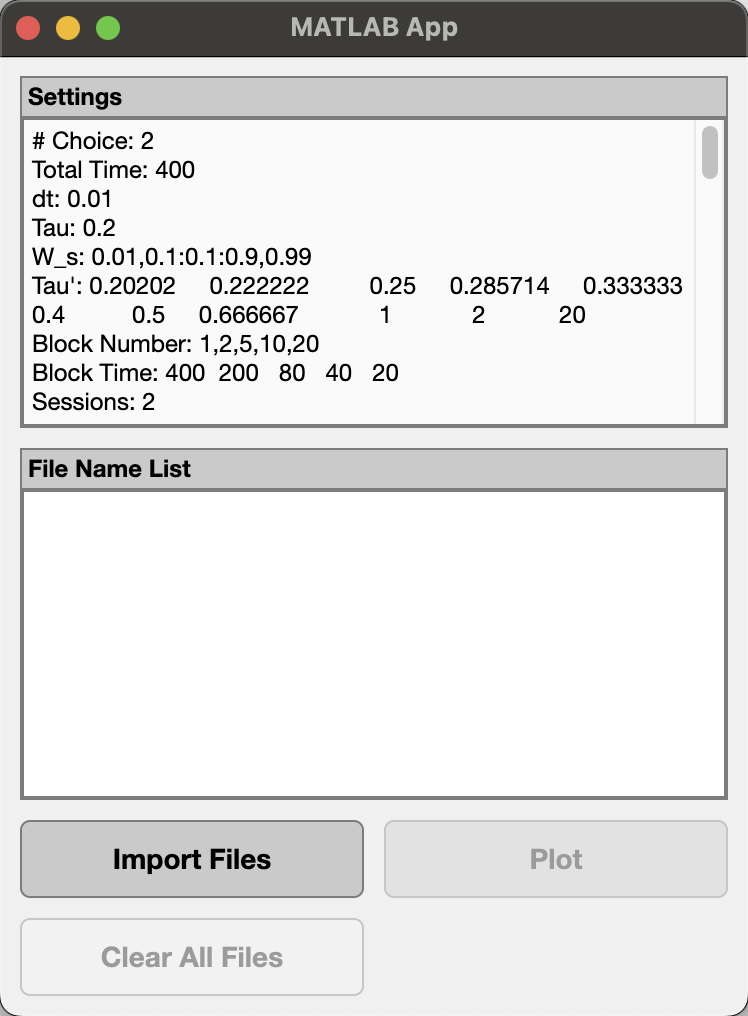
\includegraphics[width=0.5\textwidth]{figs/import_sim.png}
    \caption{Window for importing simulation.}
    \label{fig:import_sim}
\end{figure}

\subsection{Import Batch}
To import existing batch (multiple $W_s$, multiple values for another parameter, with multiple sessions for each condition) from a dataset, nativate to the \texttt{File} $\rightarrow$ \texttt{Import Datasets} $\rightarrow$ \texttt{Simulation} tab.

Similar as Section \ref{sec:import_sim}, you cannot edit individual parameter here but please go back to your \texttt{main.mlapp} to edit the settings. Here, you may select one parameter from the upper middle list box for having multiple values. Specific values need to be entered on the right side. Click on \texttt{Import Datasets} button below to select a directory for completing import similar to Section \ref{sec:import_sim}.

If at least one file for each values are imported, you will be able to check the each variable and their corresponding file name at the lower left and middle list boxes. You may also clear all the files through the \texttt{Clear imported 3D plot data} button on the bottom left.

Before you click on the \texttt{Plot} button, check the block number you want to plot, and you may switch the plotting type between \texttt{Contour} and \texttt{Waterfall} through the drop down.

Clicking on \texttt{Plot} button will also lead to open another window for plotting using existing datasets. See Section *** for more detail.

\begin{figure}[H]
    \centering
    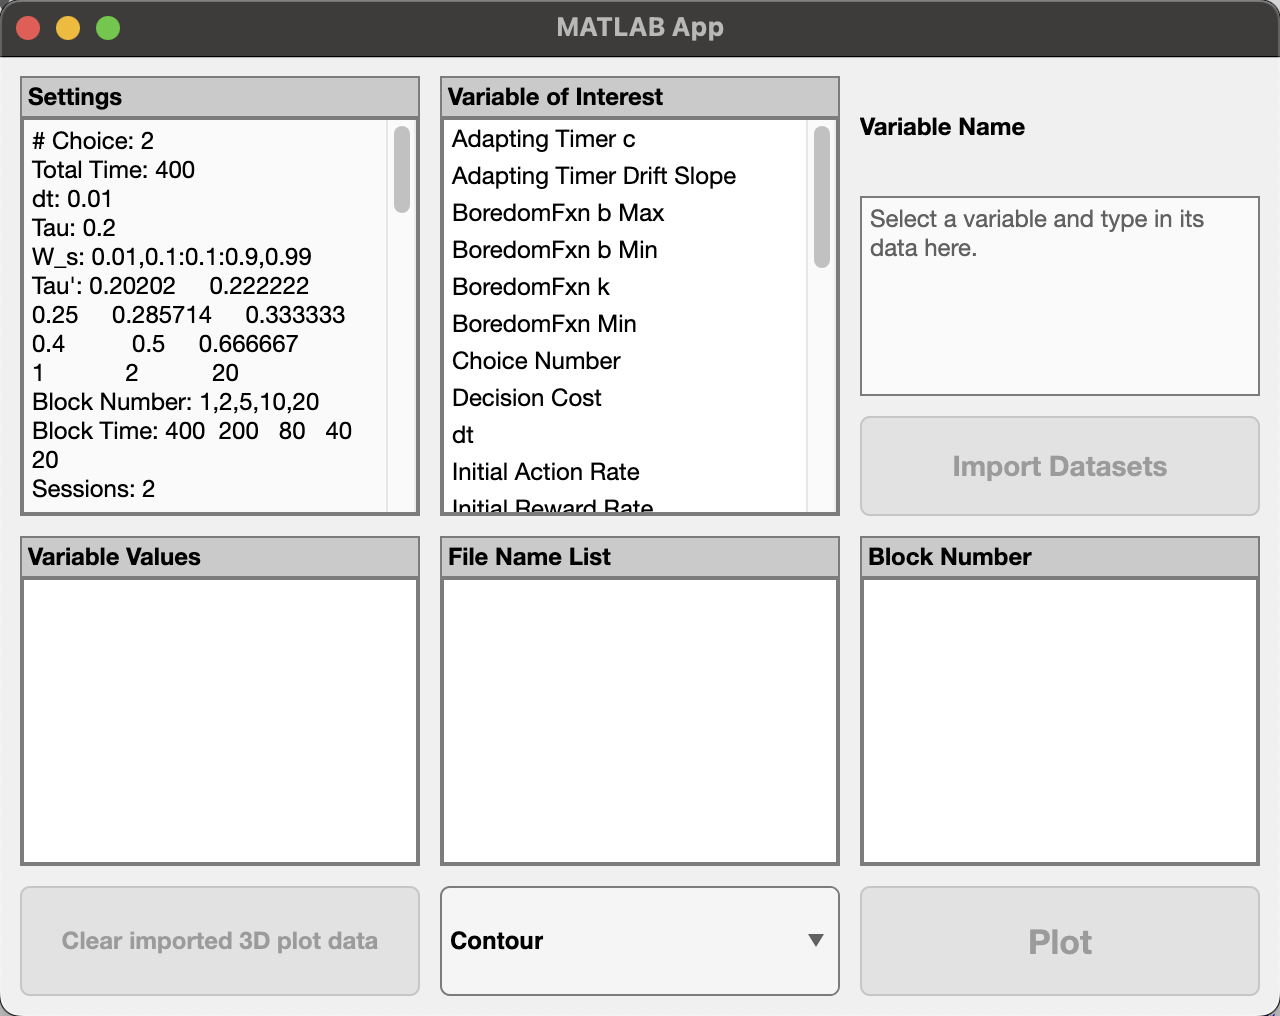
\includegraphics[width=0.9\textwidth]{figs/import_batch.png}
    \caption{Window for importing simulation.}
    \label{fig:import_batch}
\end{figure}

\section{Multiple Settings}

Since the GUI cannot terminate an ongoing simulation and may encounter unexpected errors, the Multiple Settings section allows you to create a \texttt{.mat} file for multiple simulations. You can then use the \texttt{ZeroDriftDDM\_MultipleSettings.m} script to import the simulated \texttt{.mat} file and run the simulations in batches over an extended period.



To create a batch, navigate to the \texttt{Tools} $\rightarrow$ \texttt{Batch file generator} tab located in the upper-left corner of the GUI. This will open a new window for generating the settings file.

\begin{figure}[H]
    \centering
    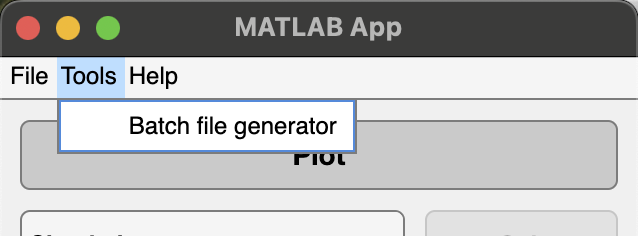
\includegraphics[width=0.5\textwidth]{figs/batch_generator.png}
    \caption{Batch File Generator Window.}
    \label{fig:batch_generator}
\end{figure}

Here you need to specify multiple values for the selected variables. All unspecified variables will retain their values as set in the general settings.

\begin{figure}[H]
    \centering
    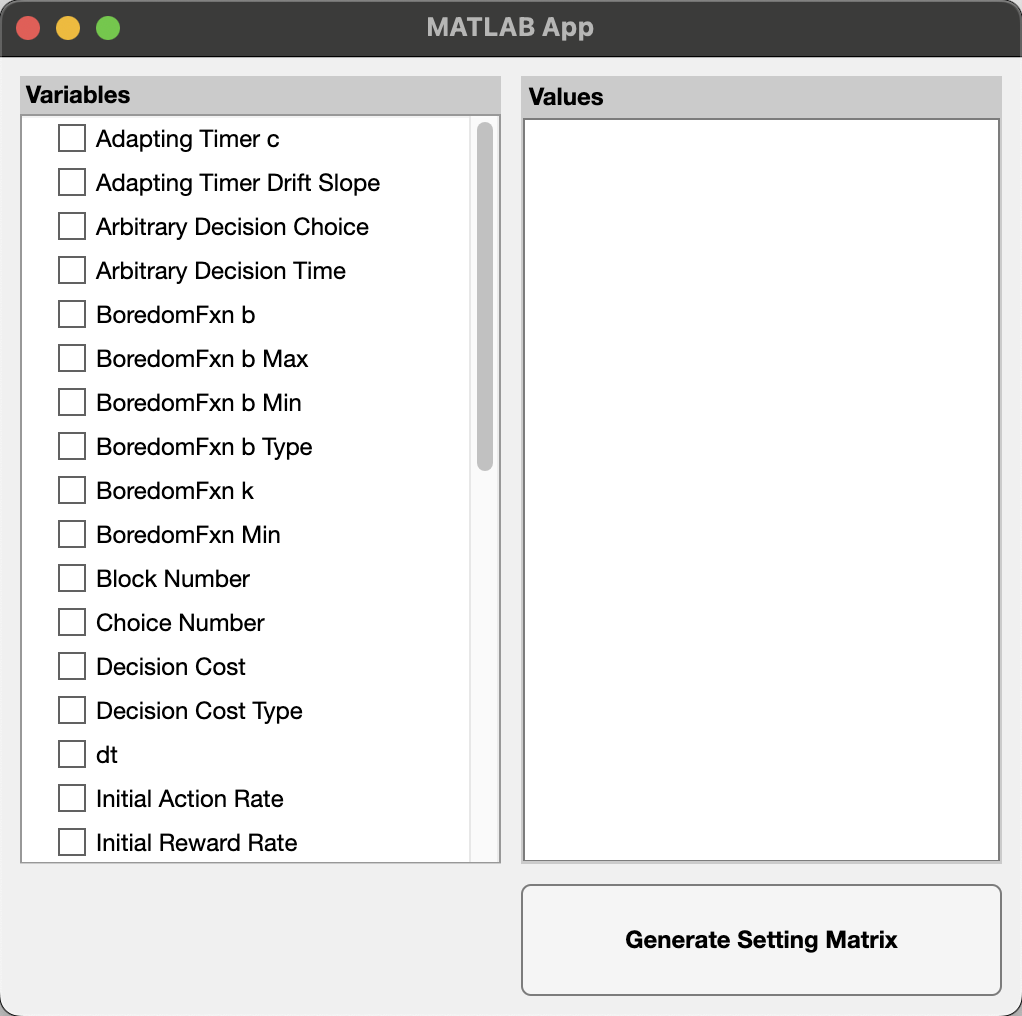
\includegraphics[width=0.8\textwidth]{figs/multiple_settings.png}
    \caption{Multiple Settings Panel}
    \label{fig:multiple_settings}
\end{figure}

For most variables, enter the values on the line following the commented variable name in the values section (e.g., \% Choice \#). Separate different values with commas.

For the Boredom Function parameters \(k\), \(b\), and \(y\) minimum values, you can either enter a single value per condition or multiple sets of values. Each set of values should be placed on a separate line. Within each set, values should be separated by commas.

\begin{itemize}
    \item Ensure that if you enter individual values, the number of values within each set matches the number of choices.
\end{itemize}

Once you have entered all the values, click the "\textbf{Generate Setting Matrix}" button to create the \texttt{.mat} file. The GUI will prompt you to choose the file path and name. Click “Save” to complete this step.

Next, use MATLAB to navigate to the folder where \texttt{ZeroDriftDDM\_MultipleSettings.m} is located. Ensure that the \texttt{.mat} file you just created is also saved in the same folder.

To start running the batch, enter the following command in the MATLAB command line:

\begin{verbatim}
ZeroDriftDDM_MultipleSettings(‘filename.mat’)
\end{verbatim}

Replace \texttt{filename.mat} with the actual name of the settings file you created.

The \texttt{ZeroDriftDDM\_MultipleSettings.m} script will display progress updates in the command line during execution, allowing you to monitor the status of the process. The progress will include the elapsed time, the current progress percentage, and the estimated time remaining.

\textbf{Note}: The estimated time remaining may not be accurate for simulations with longer total times or a larger number of total dots in later stages of execution.

\begin{figure}[H]
    \centering
    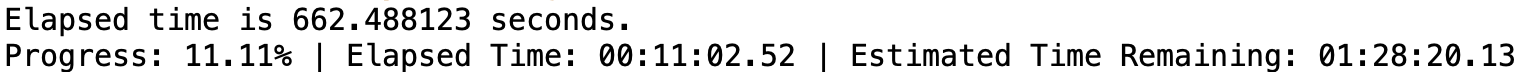
\includegraphics[width=0.9\textwidth]{figs/progress_command.png}
    \caption{Example Progress Command Line.}
    \label{fig:progress_command}
\end{figure}

\section{Batch Plot - Histogram}

The histogram panel, located under the "\textbf{\texttt{Batch}}" $\rightarrow$ "\textbf{\texttt{Histogram}}" tab, enables you to analyze the distribution of sessions for each \(W_s\) and the selected value of variable of interest. The GUI also displays the mean of the distribution, providing a clear view of its shape and characteristics. This feature helps in assessing variability and trends within the dataset.

\begin{figure}[H]
    \centering
    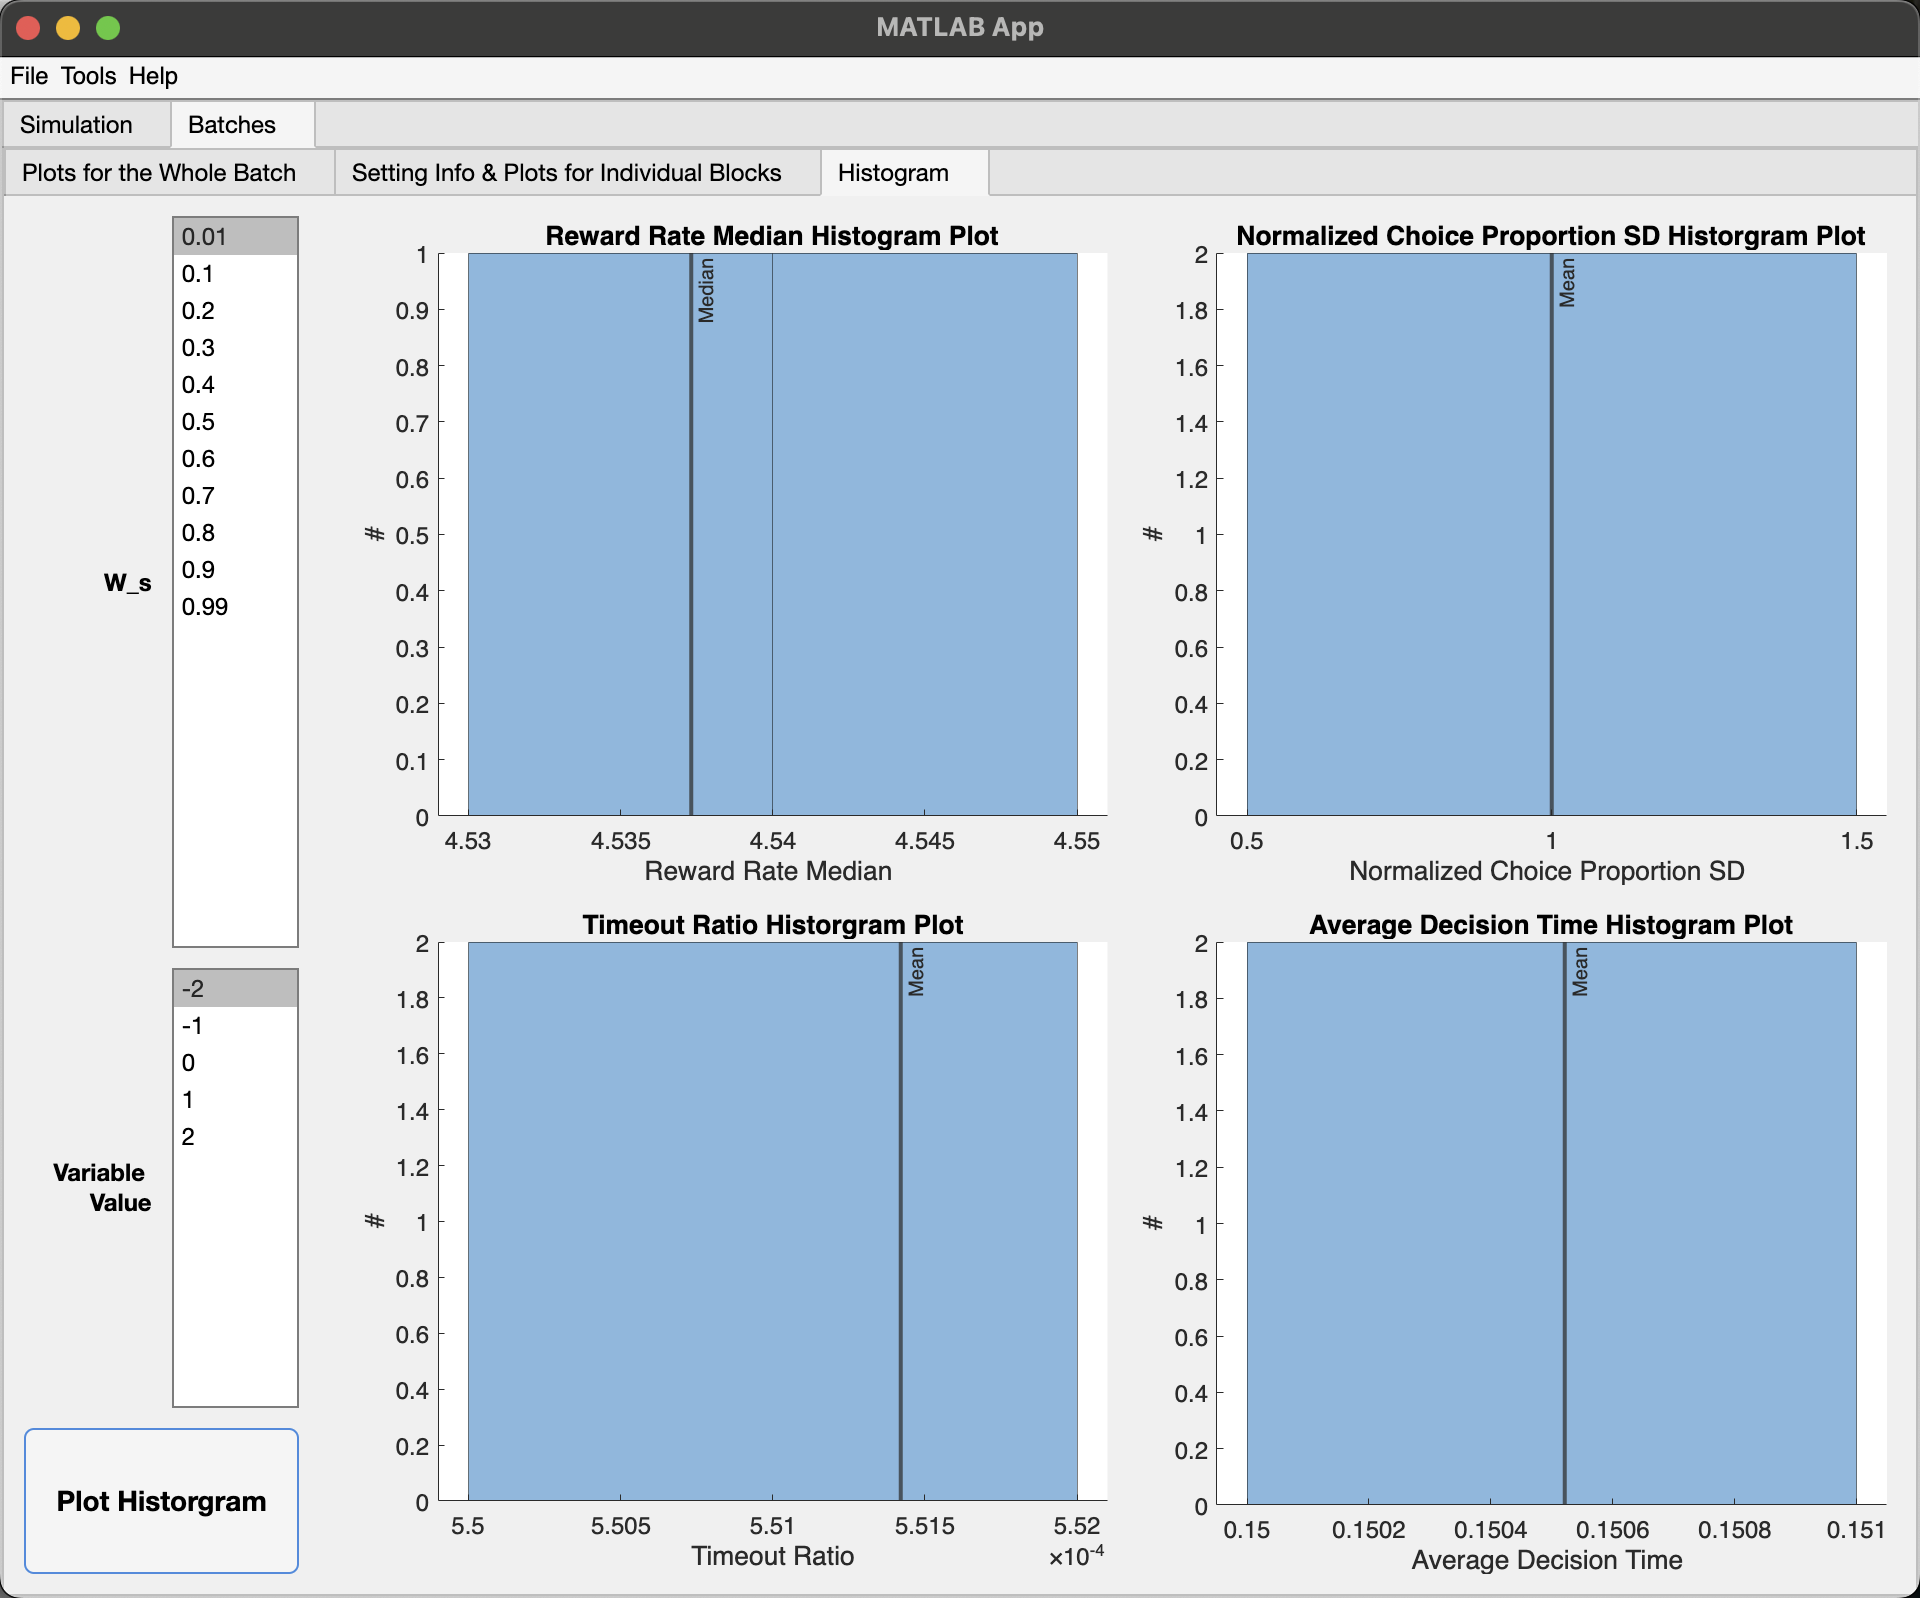
\includegraphics[width=0.9\textwidth]{figs/3D_histogram.png}
    \caption{Example of 3D Histogram Plots.}
    \label{fig:3D_histogram}
\end{figure}

\section{Menu Bar}

\subsection{Pop-out Figure}

The menu bar allows you to select a figure of interest. By clicking on the desired figure, the GUI will open it in a separate MATLAB figure window, enabling further interaction and exploration.  
If the plot does not display correctly or appears distorted, resizing the figure window should resolve the issue.  
**Note:** The colorbar will not be included in the new figure window. 

\begin{figure}[H]
    \centering
    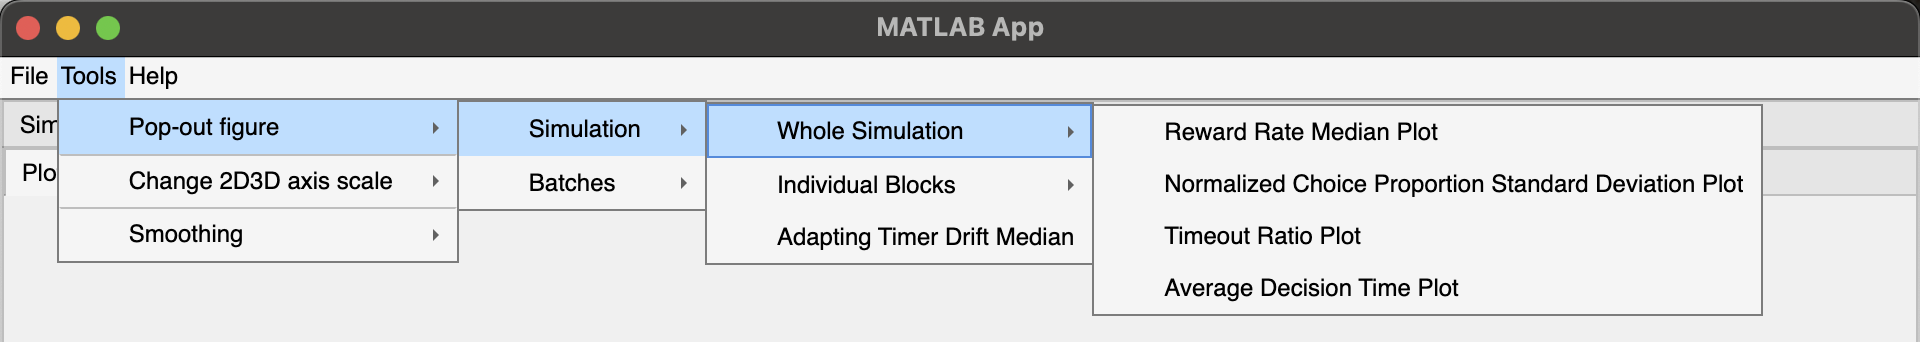
\includegraphics[width=\textwidth]{figs/popout_menu_image.png}
    \caption{Pop-out Figure Menu Bar.}
    \label{fig:popout_fig}
\end{figure}

\subsection{Save Run Results}

\subsection{Save Batch Figures}

You can quickly save all Batch plots across all block numbers as separate \texttt{.fig} files using the shortcut \textbf{Command + S} (on macOS) or \textbf{Ctrl + S} (on Windows).
Alternatively, you can access this functionality through menu \textbf{\texttt{File}} $\rightarrow$ \textbf{Export Whole Batch Plots}.

Upon triggering this action, the GUI will prompt you to select a folder. Once a folder is chosen, the following will be generated and saved within a newly created subfolder:

\begin{itemize}
\item \texttt{.fig} and \texttt{.png} files for each block number, providing both interactive and static formats for the plots.
\item A movie file illustrating the progression of changes across different blocks.
\item A \texttt{datasets} folder containing all datasets used to generate the plots.
\end{itemize}

\begin{figure}[H]
    \centering
    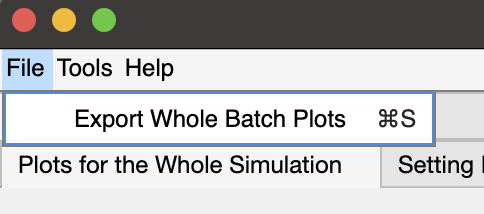
\includegraphics[width=0.5\textwidth]{figs/save.png}
    \caption{Save Figures Menu Bar.}
    \label{fig:save}
\end{figure}

\subsection{Help}
The \textbf{\texttt{Help}} menu provides access to the link to this documentation in GitHub, as well as contact information for support.